%%%%%%%%%%%%%%%%%%%%%%%%%%%%%%%%%%%%%%%%%
% The Legrand Orange Book
% LaTeX Template
% Version 3.1 (February 18, 2022)
%
% This template originates from:
% https://www.LaTeXTemplates.com
%
% Authors:
% Vel (vel@latextemplates.com)
% Mathias Legrand (legrand.mathias@gmail.com)
%
% License:
% CC BY-NC-SA 4.0 (https://creativecommons.org/licenses/by-nc-sa/4.0/)
%
% Compiling this template:
% This template uses biber for its bibliography and makeindex for its index.
% When you first open the template, compile it from the command line with the 
% commands below to make sure your LaTeX distribution is configured correctly:
%
% 1) pdflatex main
% 2) makeindex main.idx -s indexstyle.ist
% 3) biber main
% 4) pdflatex main x 2
%
% After this, when you wish to update the bibliography/index use the appropriate
% command above and make sure to compile with pdflatex several times 
% afterwards to propagate your changes to the document.
%
%%%%%%%%%%%%%%%%%%%%%%%%%%%%%%%%%%%%%%%%%

%----------------------------------------------------------------------------------------
%	PACKAGES AND OTHER DOCUMENT CONFIGURATIONS
%----------------------------------------------------------------------------------------
\documentclass[
11pt, % Default font size, select one of 10pt, 11pt or 12pt
fleqn, % Left align equations
a4paper, % Paper size, use either 'a4paper' for A4 size or 'letterpaper' for US letter size
%oneside, % Uncomment for oneside mode, this doesn't start new chapters and parts on odd pages (adding an empty page if required), this mode is more suitable if the book is to be read on a screen instead of printed
]{LegrandOrangeBook}

% Book information for PDF metadata, remove/comment this block if not required 
\hypersetup{
	pdftitle={Title}, % Title field
	pdfauthor={Author}, % Author field
	pdfsubject={Subject}, % Subject field
	pdfkeywords={Keyword1, Keyword2, ...}, % Keywords
	pdfcreator={LaTeX}, % Content creator field
}

\addbibresource{sample.bib} % Bibliography file

\definecolor{ocre}{RGB}{243, 102, 25} % Define the color used for highlighting throughout the book

\chapterimage{Images/orange1.jpg} % Chapter heading image
\chapterspaceabove{6.5cm} % Default whitespace from the top of the page to the chapter title on chapter pages
\chapterspacebelow{6.75cm} % Default amount of vertical whitespace from the top margin to the start of the text on chapter pages

%----------------------------------------------------------------------------------------

\begin{document}
	
	%----------------------------------------------------------------------------------------
	%	TITLE PAGE
	%----------------------------------------------------------------------------------------
	
	\titlepage % Output the title page
	{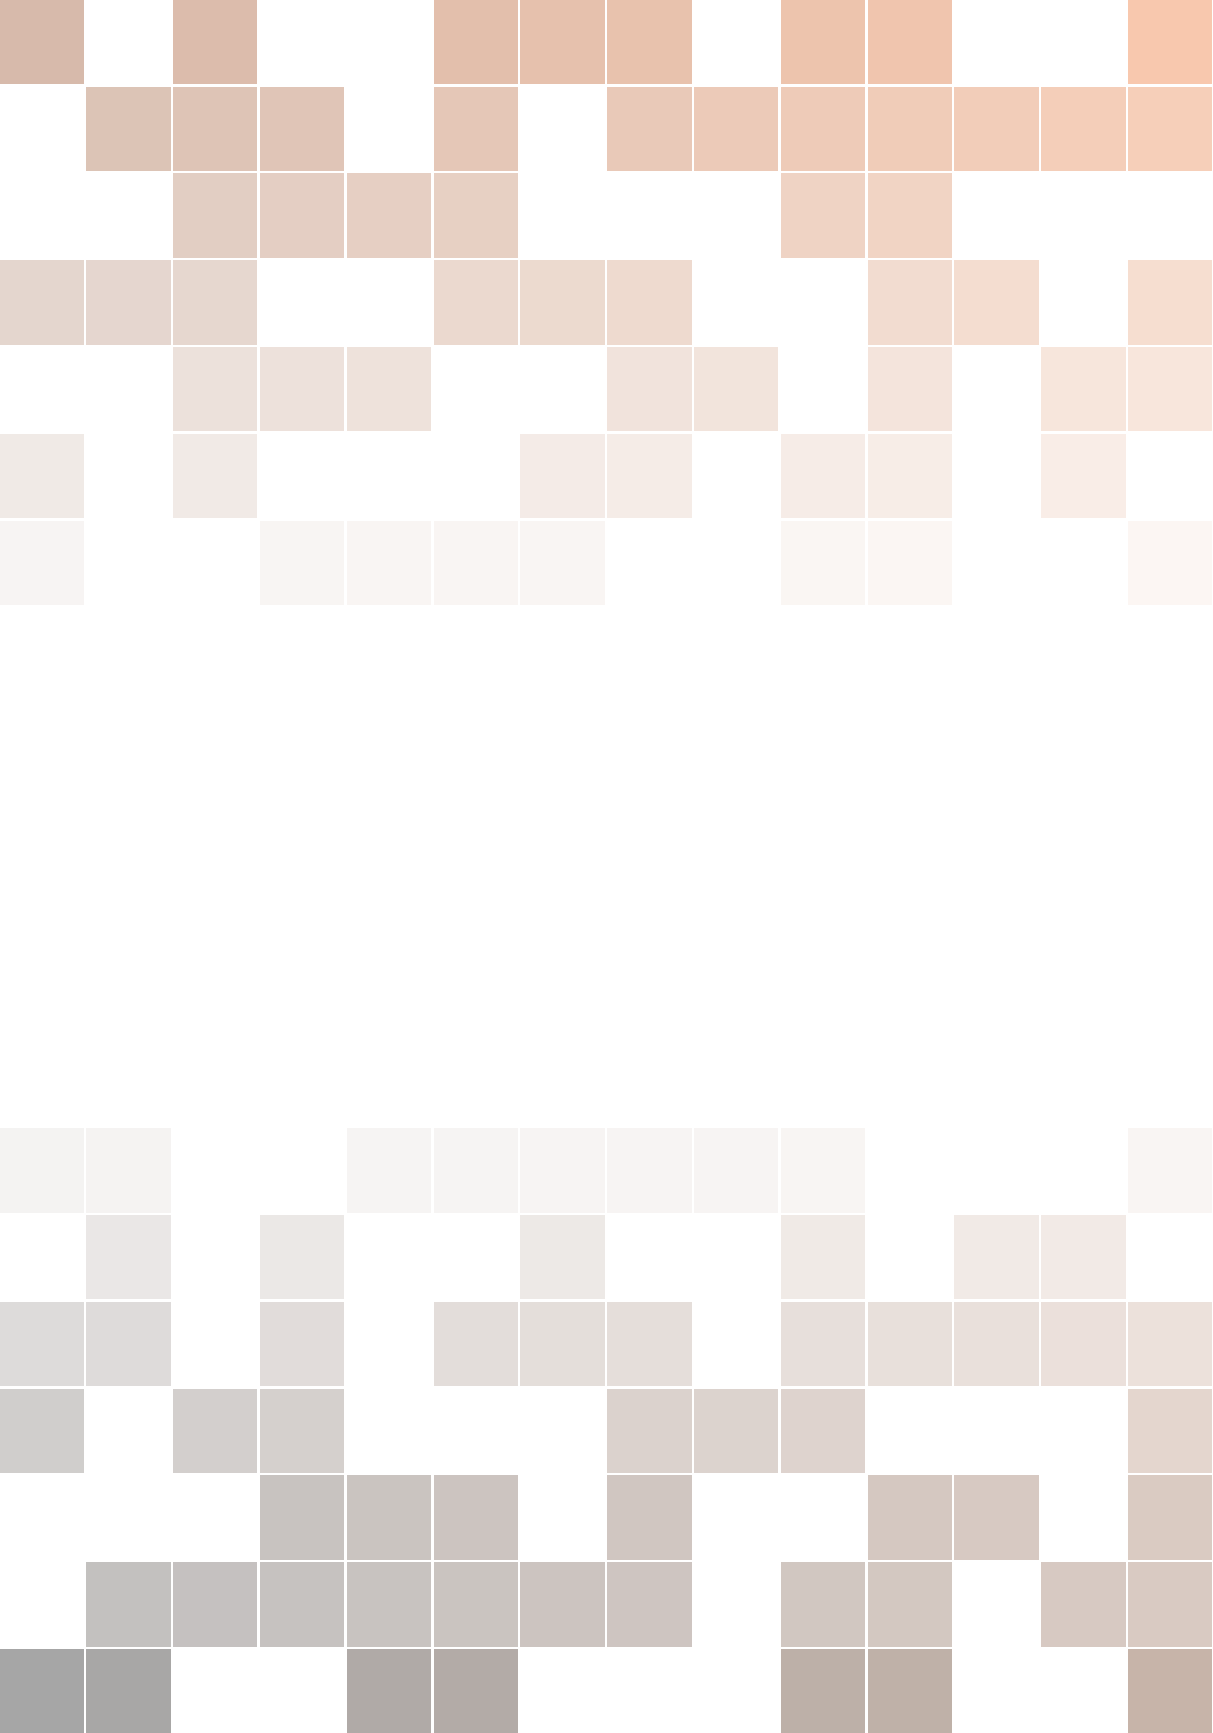
\includegraphics[width=\paperwidth]{Images/background.pdf}} % Code to output the background image, which should be the same dimensions as the paper to fill the page entirely; leave empty for no background image
	{ % Title(s) and author(s)
		\centering\sffamily % Font styling
		{\Huge\bfseries Micro and Nano Systems Track\par} % Book title
		\vspace{16pt} % Vertical whitespace
		{\LARGE A Micro Journey in a Nano World\par} % Subtitle
		\vspace{24pt} % Vertical whitespace
		{\Huge\bfseries Lorenzo Vergata\par} % Author name
		%\vspace{6pt} % Vertical whitespace
		%{\bfseries Whisper Large V3\par} % Author name
	}
	
	%----------------------------------------------------------------------------------------
	%	COPYRIGHT PAGE
	%----------------------------------------------------------------------------------------
	
	%\thispagestyle{empty} % Suppress headers and footers on this page
	
	%~\vfill % Push the text down to the bottom of the page
	
	%\noindent Copyright \copyright\ 2024 Lorenzo Vergata\\ % Copyright notice
	
	%\noindent \textsc{Published by John Doe}\\ % Publisher
	
	%\noindent \textsc{\href{https://www.latextemplates.com/template/legrand-orange-book}{book-website.com}}\\ % URL
	
	%\noindent Licensed under the Creative Commons Attribution-NonCommercial 4.0 License (the ``License''). You may not use this file except in compliance with the License. You may obtain a copy of the License at \url{https://creativecommons.org/licenses/by-nc-sa/4.0}. Unless required by applicable law or agreed to in writing, software distributed under the License is distributed on an \textsc{``as is'' basis, without warranties or conditions of any kind}, either express or implied. See the License for the specific language governing permissions and limitations under the License.\\ % License information, replace this with your own license (if any)
	
	%\noindent \textit{First printing, \today} % Printing/edition date
	
	%----------------------------------------------------------------------------------------
	%	TABLE OF CONTENTS
	%----------------------------------------------------------------------------------------
	
	\pagestyle{empty} % Disable headers and footers for the following pages
	
	\tableofcontents % Output the table of contents
	
	%\listoffigures % Output the list of figures, comment or remove this command if not required
	
	%\listoftables % Output the list of tables, comment or remove this command if not required
	
	\pagestyle{fancy} % Enable default headers and footers again
	
	%\cleardoublepage % Start the following content on a new page
	
	%----------------------------------------------------------------------------------------
	%	PART
	%----------------------------------------------------------------------------------------
	
	\part{Advanced Micro and Nanofabrication Technologies}
	
	\chapter{Magnetostatics}
The course is trying to bridge the gap between a fundamental aspect of magnetism and the real application of magnetism in real life. And I was just making this example that's been between you as a student from my group who is really working to the redesign of the magnetic field sensors. But for doing this he needs all, I'll say, all the ingredients that I tried to explain during this course. That's the reason why he's attending the course because it's not coming from physics engineering. So this course was missing in his career. A friend of mine, who's not just a friend, he was the past president of the European Magnetic Association, the name is Burka Hillebrand, who is the father of Magnolian Westerners, who is used to say that Ricardo, you have a double soul. You are a physicist but also an engineer. Obviously it's true, my degree is in electronic engineering, but in the end my PhD is in physics and I'm giving a lecture in physics. But okay, what I try in my life is really to establish sort of a bridge between academia and companies and so on, because this is our real life at the end of the day. Mathematics is very beautiful, but what is the day-by-day implication of that? Now I will try during this course to make some example which really can be used to bridge the gap to show how quantum mechanics begins real application also in the field of back end of production.\\
Basic magnetostatics, which is now the topic of today's lecture. Understanding what happens in statics. Magnetostatics means state-stage system. We are not talking about in waves, permanent regression dynamics, static configuration of a magnetic bond. which means not just iron and an infinite crystal, but a piece of iron. It is shaped as a sphere, the film, the bar, the shape makes the difference. And magnetostatics deals with the static configuration of the magnetization, not the field created by the magnetization. In some sense, this is the physics of three magnets. Okay, when you have a three magnets, you can play with magnets. And you know, if you know this game, which is your mind. You're playing with German. Yeah, that's a good starting point for this. Get to play. So you understand the magnetic force magnetism. And what's your name? I sound good. That's the names of today. It's been so let's start with when you play with the German. I give Pearson is the right-hand pole, he is the left-hand pole, North, North, and South Pole. So we have to understand the physics of the geometry. Okay. First of all, let's review which are the main characters of this course and the basic equation that you have.
\fig{2}{lecture_1 basic magnetostatics.pdf}
So you have different characters and things. B, H, and L. Okay. Well, the three guys are feeling this one. B is the induction field. H is the magnetic field. M is the magnetic solution. Let me just review the meaning of this. Which is the difference? Sorry. I apologize. I apologize. M is the magnetization. What's the definition? It's the magnetic moment that you are holding. Magnetic moment that you are holding. So what does it mean? How do you measure a magnetic moment? Magnetic moment, you should always refer to the idea of the circuit, so the magnetic moment is measured in water. It's the intensity of the current multiplied by the area. And when we go to the magnetization, we need to realize that magnetization is measured in water. Current by surface divided by volume, to the current divided by a light. That's why in terms of units, it is measured in amps per meter. That's the unit of the magnetization of the International System of the Universe, in which we will live and be. I made this choice in the very beginning, not purely for the different systems that I'm using in physics. I'm using now the International System of the Universe. amps per meter. And then you have the induction field B and H. I ask you, what is the difference between B and H? I do not completely agree. the example for HF. Okay, the relation is this one. B is equal to 0H plus F. Okay, that's the definition. But physically, you have to say what is the difference between B and H. But for that, B is the vector appearing in the Lorentz field. So an electric charge is moving in a magnetic field with the Lorentz force, 2B cross B. and is B the field which determines now the force acting on the magnetic field? It is B. H is something slightly different because H is connected to what? The current. The connection is quite straightforward. You know that the curl of H is equal to J Not only this, but what should I have here? Maxwell equation, one hundred most beautiful things of every size, plus, plus root. Something is missing. Yeah. You can write in the free space or otherwise you can write in the derivative of D, with respect to the time. But for today, if you write in magnetostatics, you can also forget about this one. Magnetostatics means the states of the oscillation of the coordinates of the light and the field is not changing. But you immediately see that H is directly connected to the source of the magnetic field, which is usually connected to the current flowing in a wire. But this is not the unique vision of the story, especially magnetostatics, also because when the free space but their current amount, no. Obviously, the field is going to be better. And what is now the problem or the opportunity? The opportunity is here, B, as you see, the museum, EH plus M, okay? So, and the H can be reduced by the magnetization itself. So, what is the Fritz magnet? The Fritz magnet is made of an odd magnet, typically a cobalt, a boron, or a chloride, which displays a nice, realistic look. So, at zero, external field, you have a net Riemann magnetization. And so, this is the source of the H, okay, especially magnetostatics. In magnetostatics, when you say What does it mean? There are no currents of one in the center. That's the framework in which we are more. So the the derivative we expect to time are equal to zero and no current. So the sources of the magnetic field are not connected to cards, but connected to the presence of the body which is magnetized in remnants due to the fact that it's a full magnet due to exchange interaction with a remnant magnetization at zero external field. And that's the reason why when you move from there to this relation here, you usually find that B is equal to mu zero, HM plus M. And this subscript M is here just to tell you that this is the H field not produced by the current here. The J zero here, okay, is produced by the magnetization itself, okay? So no current means that the H is not produced by J. So this means also that the curl of H equal to zero. Okay? This is zero. And that's the reason why in magnetic structure, at values with the general framework of electromagnetic you can define what is gamma retention. The reason is quite heavy, it is immediately evident. If you see that you have a vector h whose curl is equal to zero, but this means that you can write h as the gradient of something else, a kind of field, exactly as in order as in order to start. So you can say that, okay, so if this is the story, I can write immediately H is equal to minus the gradient of a scalar potential U. Usually you cannot do that. So the kernel of H is equal to U, not because we are trying to use the vector equation. But this is not the case. Here you can use a standard equation. And there is another story which is also relevant here. In terms of units. I didn't feel completely stable here. M is the magnetization which must be expressed in m per meter. But according to this equation here, here, m and h, they have the same units, okay? This is quite evident. So h, again, in amps per meter, so if you want this magnetic field, and this is the induction field. and the magnetic field must be measured in m per meter and as you have this pointed here this constant which is near zero which is the back of the mobility 4, 5, 8, 10, 11, 17 units in the initial system it does all that it also has it's not dimensionless this one So then the unit for B is Tesla, okay? In the international system of units. B is measured in Tesla, M in the international system of units. Okay, so these are the three characters of magnetostatics. The basic equations are these two equations here, and from these you immediately realize that you can use the scalar potential, which is much easier for multiplication. Scalar potential. And now, what's the impact of this? Immediately you realize that you can apply the same mathematics over the rhythm of statics. So we have the scalar potential, h is minus the gradient of u, which is like the case of e, given to e, but minus the gradient of p. And so, okay, and so. And so what happens? You can say okay, but if you have this equation here, you immediately find that you can write down a Poisson or Laplace equation for the magnetic star hypotension. And how it goes out? So it's very simple. So do not forget that B is always true that the divergence of B is equal to zero. Because there are no magnetic monopoles. The divergence of B is always C. So essentially, you have it, okay? The divergence of B is equal to zero, but B is mu zero by H plus M. This means that the divergence of H is equal to minus the divergence of M. Okay? And then instead of H, you can replace minus the gradient of U, and this means minus the number of squares of U, which is equal to minus the divergence of M, and so your your language with this equation. The Poisson equation, okay? The Poisson equation is the number of squares of Q which is equal to the divergence of M. It's very similar to something that you know. Number of squares of B is equal to minus O divided by epsilon Z. Okay, it's again a Poisson equation. And so from the analogy that I started to tell you about, this seems to be related to sort of charge. And indeed we will see that it's exactly connected to the concept of magnetic charges. But okay, let's continue this discussion. So we are here, we have this equation here, It's a sort of Poisson equation. Inside the magnetic body, you have a diagonal. You have an M, okay? Don't forget that in general you have a magnetic body with a volume, surface, and the norm under the surface, N, according to this. And inside the body, you have a non-moon diagonalization, so you can have a 30-D-L. It can be zero or not, depending on the divergence of M. But you can have it. But outside the magnetic body, there is no M, M is zero, the divergence of U is zero, then you have not a Poisson equation, but a Laplace equation. now the square of u outside must be equal to zero. And now you have this Laplace equation plus some equation. That's a typical problem that we have seen in electrostatics, and so one can say it's the answer. Of course, we have some boundary conditions, because we have an equation inside, an equation outside, now without the boundary conditions. We will see afterwards that the boundary conditions for U at the surface are these two conditions. The continuity of the U is very similar to the continuity of the electric field. The electric field can admit this continuity, not the tension, otherwise there is a divergence. And there is another condition, which is this one, stating that if you calculate now the derivative, the direction of the derivative, the derivative of u with respect to the direction to the norm of the derivative inside, you subtract the same direction of the derivative outside, immediately inside, immediately outside, this is equal to m dot. We will see that this is exactly the same condition that you are used to, stating that the normal component of B must be conserved when you cross a little bit between the two points. But okay, you have this regulation, and you have this binary condition, and provided that you find a solution which is regular at infinity, which corresponds to this condition here, condition, a fantastic condition, a fantastic situation, so that if by inspection you find a solution, that the solution is not a second solution. This genus theory is an extremely powerful tool for solving magnetic static. And this is a very powerful method for solving the problem that we will see.
\fig{3}{lecture_1 basic magnetostatics.pdf}
Now, as I was telling you, this is a negative sign. That could be also an exact sign. That's exactly this one. So, demonstrate that the boundary condition that you are used to from general courses of the electromagnetic state in that when you cross an interface, the parallel component of H and the perpendicular component of B, not B, show that these are equivalent to the following conditions, exactly the conditions I told you about. So let's solve this exercise, just to work it out. So one could start with the condition for the conservation of perpendicular components of B. So what happens? Let's imagine that you have neutral states between two magnetic materials, different magnitudes. This is inside, so let's imagine that, okay, this is your body, okay, so you are here, and here it's outside, okay. So the typical story that you know is that inside and outside the perpendicular component of B must be equal. So B in perpendicular must be equal to B out, okay? This is B. But now what about B? B is mu zero by m plus h. Inside you have m, outside you don't have m. So this is your body, outside you have a vacuum, but it's no magnetic material. So inside you have to write down mu zero m plus h m. Okay, inside. So, outside you have what? Mu zero, h m, no longer there. So mu zero, you don't need it. And now you have what? Okay, m. But you have to take what? The perpendicular component. So this gives y. So you take the projection on the normal, the unit vector which is normal to the surface, which is n. So let's assume that here you have this n. So you take m dot m plus volt. Okay, let me say that this hm can be written like minus, what is it? H is minus the gradient of u inside. So you have minus the gradient of u in dot m, u in dot n, which is equal to h outside, same story, minus the gradient of u out dot n. But when you take now the scalar product between the gradient and the normal, what are you find? r is the direction of derivative along the direction of the norm. You project the gradient in the direction to find the partial derivative along that direction, to the So, in the end, you have m dot n. So what is this? Minus partial derivative of u in with respect to n, equal to minus partial derivative of u out with respect to n. And this is exactly the condition which is reported there. So in the end you find out that the discontinuity and the partial derivative from inside and outside is equal to m dot n. Okay? Good. First condition, which is demonstrated, so the equivalence is demonstrated. you have a cycle one just that concerning the fact that the parallel component h in parallel might be concerned but be equal to h out of that and here i say what you say it is automatically satisfied i told you that h is equal to minus the gradient of U but okay this means that the curl of H is 0 okay no way curl of H is equal to 0 if the curl of something is equal to 0 it's very easy to demonstrate that you take a path like this and you integrate the curl this means the circulation over this line must be zero, and this automatically brings you to the conclusion that the true pilot component must be equal. Automatically . And then, what's the origin for the continuity of the U inside and outside? It's not connected to a very simple show. As H is equal to minus the gradient of U, It's evident that if you have a discontinuity in the U, you will have a divergence in H. And you want to avoid this divergence, which is unphysical. It's exactly like an electrostatic. In electrostatics, you can have a discontinuity in the electric field, but not discontinuity in the potential. So if you are discontinuating the electric potential, there is a divergence of the electric field at that boundary. here is exactly the same thing. So when you write down these conditions, you ensure that H is according to which is well defined without divergence, and you are ensuring that the parallel component of H is conserved and what's the curtain in your component is conserved. Okay, so this is an exercise that I'm used to to solve. Are you okay? What's the name? You also fear that you won't qualify. Sorry, just trying to recognize the face. So, it's an exercise just to make some practice with Maxwell equations, which could be also nice for restarting a little bit at the beginning of this course. OK, but now what's the point? We found that we have an equation which is nice, which is an equation in which you are essentially look at this part here.
\fig{4}{lecture_1 basic magnetostatics.pdf}
It's a Poisson equation. This slide is meant to establish a full analogy between magnetostatics and electrostatics. Look, for the magnetic material, we have that B is equal to 0H plus M. For a dielectric, we have that D is equal to epsilon zero by E plus P. What is P? is the polarization effect is measured in two more room meters squared. And so you see that there are three characters with some correspondence. So B, the meaning of D, the electric field H, and instead of M, you have B. And those are physically you understand that the meaning is very similar the polarization that you can have in the material has the same function the functionality of the magnetic solution and as a matter of fact the equation described in ferroelectrics and true magnets are very similar the long dowel potential for both systems is exactly the same so the same properties can be you have a coercive field, an inferred magnetism, an electric field, you have saturation, remnants, you have a coercive field and also a loop, an integrated loop, anyway. Now, H is equal to minus, gradient of U, but E, the derivative is minus the gradient of H. One to one. There is a difference. The divergence of B is zero. That's a big difference. the divergence of E, the Gauss theorem, is equal to the density of charge divided by the density of E. But in terms now of the equation that you find, here you have the number square of U, which is equal to the divergence of M, and in that case, you have the number square of B is equal to minus 4 divided by absolute E. So, let's use now the thermo-centrifugal climate. The same equation has the same solution. How can you apply this central theory? Because, okay, what are you used to apply in eletrosclerosis to solve the problem? You say, okay, I have this equation. Now, forget about the left problem. Now, the density of charge that we put there is the sum of two contributions. We can have three charges, those appearing at the surface of the components, and polarization charges, those appearing in dielectrics, either at the surface or even in the volume, depending now on the condition of polarization of the volume. But what is the solution for the problem of the electrostatic? We can write down the expression for the potential, starting from the superposition principle and the solution for one charge. So that you can say that as the source for the electric field are water, the potential, the free charges on the conductor and the polarization charges, we can write down this equation saying that okay the road to be placed here is the sum of three row three density of charge minus the divergence of the example is the way you write down the density of polarization okay so let's assume that row three is see what you see. I'm not coming back to it. So I just left with a dielectric material which is polar. It's exactly what you have on this side for the main of the star. You don't have electric current here. The equivalence story is we don't have electric charges to the mass. So, the Poisson equation becomes the number squared of V is equal to minus by minus the state of space plus the divergence of space divided by epsilon. This is the equation, and the solution is something that you know very well. The solution is this one. V is equal to one divided by four pi f multiplied by one, the sum of two into one. The first one is the contribution to the electrostatic potential coming from the volume of the charge. C minus the divergence of P in the R-th parameter, divided by R minus R-th, contribution from the volume charges of polarization, plus the contribution from the surface charges of polarization, P dot n. Okay, this is the really the surface density of collision charges divided by r minus r prime integrated over x. This is the solution of the equation. But now you can say, okay, the density, the volume density of collision charges is minus the derivatives of p and the surface density of collision charges is p. Now you go back and say, okay, but here I have this equation and the other equation. So now you can say, okay, same equation, same solution. Strong parallelism, you say, okay, let me write down instead of v, u. Here you have 1 divided by 4 pi epsilon zero. Okay, here you have epsilon zero, here you don't have something at the denominator. So just 1 divided by 4 pi, multiplied by the sum of two integrals. The first integral would be a volume integral, same here. divergence of P, but P, in this case, is m, so minus the divergence of m, divided by r minus r prime, integrated over the surface. Then you move to the integral over the surface, that was here P dot m, what do you find here? m dot m, divided by r minus r prime, integrated over the surface. And that's the solution for U. You see the strong analogy between the two things, same equation, same solution. So you have found now the connection between the magnetization and the U. And the problem is solved once forever, because now if you know the distribution of M, you You can calculate the U and if you can calculate the U, H is equal to minus the gradient of U. End of story. You see my point? The problem is solved. And now there's another column. Do you have a question? Yeah. I'm not sure. Yeah. It's another idea. Right. Is the analogy so that when we are talking of charges in the dielectric field, the corresponding is the charges and the corresponding is current. Exactly. So, by analogy, volume and energy charges are current in this case. Are you referring to this slide? Yeah. So you're asking me something before I explain that. Just go. What is that? I have something. I have something. I have a signal. I have something. Okay, one neuron remains. It's a big issue. Sorry. Okay. Let me first make a comment and then probably the solution, the question, the answer to to your question should be quite clear. Let's now make a comparison between this solution for U and that solution for V. You immediately try to associate this minus divergence of M with the minus divergence of P. But as minus divergence of P is the density of polarization charges, You introduce this concept, which is a pure mathematical concept of volume magnetic charges. As you see, minus the radius of P is physically a volume density of the partition charges. Okay, so this term, BA, is like a volume density of something that I call by analogy magnetic charges. Do magnetic charges exist? No. It's just a pure mathematical concept that you are using in order to explore the analogy. Okay? They do not exist. So the divergence of B is equal to zero. Okay? only the Naomi dipole exists so far, okay? Who will demonstrate something else with the normal price, millions of dollars, for the time being, is pretty much equal to zero. So this means that it is just a mathematical term that is useful and can be helpful when you try to solve a problem, but it's a mathematical term and by analogy. What about m dot n? p dot n is a surface polarization charge density. So you say that m dot n is like a surface magnetic charge density. Okay? Why it's so relevant to your theory? not everybody loves this kind of approach. People say, okay, now you have to use the vector potential in a way, why are you running with the scalar potential? But in practice, you will see in a while that establishing a sort of parallelism, like the static problem, ending with a static one, is very powerful because it because it provides you with an immediate vision of what is going on in the magnetic field, starting from the concept of the electrostatic process. You know very well, you are not used to work with magnets, you are more used to work with electric charges, potential and so on, so you can now use what you know from the electrostatic and apply it to you. That's more or less the A very simple example would be this one, and then we will take a break, otherwise the lecture will become too long. So you know what's the origin of magnetism, of the name magnetism? You know the origin. You know magnetite. Magnetite there, okay, what is magnetite? It's a rock, okay. So magnetites come from magnetite, okay, but which is not the end of the story. to magnetize In iron free Is a rock but who gave the name magnetized to this rock With bricks they did they gave the name to her to everything They just they discovered everything and also the final that we were just making something final everything was done by greeks So yeah, the Greeks, which Greeks living in which city? Is he famous? Was he a philosopher? Okay, but he's connected to Magnetism. It's Magnesia, the city of Magnesia. Magnetism comes from the city of Magnesia, Magnetism comes from the city of Magnesia, in Italy, the station of Magnesia. And that magnetism came. They discovered the property of this rock around the 7th century B.C. And they were typically playing with this rock shaped in the form of a bar. Like in the German. For a reason that I will explain in a while, when you have a bar or a through-magnetic body, it displays a natural tendency to develop the remnant magnetization along its axis, Which means that you can imagine that M is uniform and is directed along the axis. But now let's imagine that you have a cylinder which is uniformly magnetic. Quite low. Do you have some magnetic charges inside or at the surface? Let's imagine that it is uniform. there are no volume magnetic charges, so the divergence of M is 0. No magnetic charges inside. Are there some surface magnetic charges? So you have to calculate M dot N. And now you have two possibilities. This is N here, but M dot N is 0. zero, you don't have magnetic charges on the surface, on the lateral surface of the cylinder. Nothing. Zero. But what happens here? Here you have N1 and here you have N2. And you discover that M dot N1 is positive and on the other side you have sigma 2 which is m dot n2 which is negative. So you can now say that mathematically you can think about some positive magnetic charges here, some negative can be charged there. And now let's imagine that you have a problem like this in a leg of a car. Which kind of field do you expect to see? You know the solution. The field lines are expected to be like this. Which is exactly the solution for the magnetic field produced by a valve end. That's the reason why he played with the German. Because if you have a cylinder which is uniformly magnetized along the direction of heat, Hartz's, you just have some magnetic charges concentrated at the two extreme portions, at these two phases. So these are the the north and south poles interacting differently, okay? Positive and negative charges. Two positive poles, they repel each other. Two poles with opposite sides. But, I think it's exactly this. And this is just a pretty simple example explaining why disposable magnetic charges can be very, very helpful. We will review his many, many facts, but from now on, we will leave it. quantitative and elegant way.
\fig{5}{lecture_1 basic magnetostatics.pdf}
So essentially we have the problem of an infinite cylinder with an axis along z in this x, y, z reference frame. And let's assume that the infinite is physically, unphysical, but it's a mathematical simple problem describing a long cylinder. It is the same that I just tried to solve here, in which we are putting the charges far and far away. Now M is uniform in size. It means you take the magnetic material, you shape it into a cylinder, you magnetize it in the Z-direction and okay, the problem is there. Which is now the magnetic field. The B is H, produced by this distribution of magneticization. So we know that the equation is always the same with the Poisson equation, but in this case, as M is uniform inside, We can't argue that there are no quantum magnetic charges, that the Poisson equation becomes a class equation. The number of squares of u is equal to zero. And the general equation of this is what? The number of squares of u is equal to the divergence of m. But as m is moving from the inside, the radius of m is 0, and we are left with a log-Nagel situation. Clearly, in this case, it is useful to work in cylindrical coordinates. The double-square assumes this form. When you are using rho, which is the radial coordinate, phi, which is dv, the azimuthal hangar here in the x-1 plane, and z, of course, which is the coordinate of the axis of the plane. So this is the representation of the Laplace equation, and what about the boundary conditions? Boundary conditions here are connected to the possible presence of modes of magnetic charges. But in this case, you don't have magnetic charges. reason is quite simple, because m dot n is equal to zero, m dot n, they are perpendicular. So there are no magnetic charges on the lateral line of the solution, okay? No charges there, and in this case, there are no magnetic charges at the top and at the bottom, because at the top and the bottom, they do not exist. They are an infinite cylinder, or they are put at infinite So boundary condition becomes this one. So there is a continuity in the partial derivative with respect to the n, which is the body of the constant. And you know that you must have a complete condition. How do you solve this equation? Don't forget that if the solution exists, it's unique. What is the trivial solution of that equation? Respecting the boundary. U equals the constant. Okay? Because if U is equal to the constant, perfect in the sense that, okay, the equation here is partial derivative equation, equation, the automatic density is zero. And, of course, the two partial derivatives equal to zero, and there will be a continuity of the U from inside to outside. So, immediately you find that this simple solution that you see by height, by inspection, is U equal to zero. Okay? And now what is the implication of u equals to zero? What are you looking for? You're looking for h. h is minus the gradient of u, which is equal to zero. So what's the implication? h is equal to zero everywhere. Okay? Everywhere. Does it make any sense to you? You have a material which is uniform and magnetized and if it is linear and H is equal to zero Is it possible that it makes sense? Or some Is Can you find any connection between this problem and that problem? This one. This problem transforms into that problem if you do what? If you put these two faces at minus infinity and plus infinity. But what's the impact? We have magnetic charges at infinite distances that do not create a magnetic field where we are. You see? But in case of the 11th time, if you have some elliptic charge that place at plus infinity and noise infinity, it will not produce a 5, it will be a ui. You see the point? So it makes sense. Here, it makes sense. So you have that H is 0 everywhere. What about B? Is it 0, B? No. So, B. So, H is equal to zero, but B is equal to mu zero H plus M. So, you have B is equal to mu zero M. So inside the cylinder, you have m and you have b, and they are parallel. b is equal to mu0, but we don't have h. So h is equal to 0, and h must respect the statement as the surface, there must be a continuity in the parallel to the point of h. If h is 0 inside, it's also 0 outside. But let's go back to the other. This is for an infinite cylinder. And in that case, in the previous one, this was H out. What about H inside? In the case of a finite cylinder, H inside. could be now the orientation, the direction of age inside? What's your name? Sorry. Eduardo. Eduardo. What do you mean? From right to left or from left to right? But so it all this proposed in like this age in Do you agree What's your name Why do you say the opposite you have to H parallel inside and outside, they must be equal. So it's impossible to add this. You see my point? That's impossible. Because this will violate the conservation of the tangent of the parallel component of H. So, H inside would be like this. And this is totally coherent with the analogy with electrostatics. Because in electrostatics, the electricity goes from positive charges to negative charges. And in magnetostatics, it's exactly the same. The magnetic field H goes from positive charges to negative charges, both inside and outside. So this is the unique possibility that you have. Pay attention to one fact. H inside here opposes the magnetization. That's the reason why it's called demagnetizing field. the fact that you create a surface, it creates some, so you're creating some magnetic charges at surface, and they generate a field which opposes the magnetization. It's a demagnetizing field, which tends to demagnetize your body. Okay? Okay. So coming back here, that's the reason why you say H in is also called H demagnetizing or HM or H in. Demagnetizing field, magnetostatic field produced by the magnetization or H inside. Just different names. But this is a very fundamental concept. So there is a demagnetizing field, which opposes the magnetization, due to the fact that you have some surfaces. You have a finite volume to be applied by the magnetization. In case of the infinite cylinder, there are no magnetic charges, so, the charges are plus infinity, minus infinity, they are not able to create a demagnetizing field here that's equal to Z. So then B is equal to mu zero by N. So in this sense, the maximum B that you can have is that for an infinite cylinder. Because you are during the demagnetizing field. Okay? And then, okay, there is a strange story here that we have to review in a while. Let's see, so EM, what is EM? EM stands for magnetostatic energy. Something that can be seen is that the magnetostatic energy in this case is equal to zero. I will try to review this concept afterwards, after explaining in more detail what is magnetostatic energy.
\fig{6}{lecture_1 basic magnetostatics.pdf}
Let's solve another problem. Just very, sorry. Yeah, this one is very similar to the previous one Jogging is exactly the same In your infinite cylinder that you're ready to are but now it's my it is magnetized along X direction to the right of it Big magnet and the other song and the top three it can be my reward the magnetizing on the x-axis. But now what's the field produced? Are these perfect or not? The question is completely, but now you expect to see some magnetic charges on the moon. Now same machinery and you say okay So this is the first case second case here Nothing changes here. Okay again M is uniform inside which means that the equation is always the same Yeah, then Navla squared of U is equal to 0 now the boundary condition So the equation is always the same but the boundary condition are different The boundary condition is the boundary condition are expressed like this So Let's me do something This X is Y and then this point towards you. Okay, so this is a cross-section In your circle radius are So it's not very good The magnetization is Pointing please This is m. Okay. And now, let's write down the boundary condition. Boundary condition is saying that the derivative of u in psi with respect to r does it... Let me say that, for instance, I'm taking this angle, which is the angle phi, the n as a normal, like this. Okay? And so when I take the partial derivative with respect to n, I'm taking the partial derivative with respect to the value of the insulated asymmetry. So it is the partial derivative with respect to n inside, minus the partial derivative outside, with respect to r, must be equal to m dot n, okay? What is m dot n? It's m by the cosine of the angle of 5. Okay? m by the cosine of the angle of 5. Now, we are left with this boundary condition, and And so one could say u equal to zero cannot be a solution. It doesn't respect boundary condition. You will have zero equal to something that is not zero, not everywhere, so it cannot be a solution. And by inspection, we can easily find that a solution could be this one. I understand that you have the light here is creating some problems, so let me provide solution, so the u, the function of r, can be written as ms divided by 2 with, okay, now, the nightmare for you, being kind of in here anyway, there's no problem. So ms divided by 2 by the cosine of the angle phi, okay? And now, if you are inside, inside the cylinder, you multiply by half, by rho, or by half, same story. Or, you have ms divided by 2, again cosine of phi by r squared divided by r. Okay, in case r is larger than capital R. And you find it's a solution, it's quite easy. If you replace this one inside the equation, you find that it is . equation, which has the previous substitution and so on. But now, if this is a solution, what is going on? First of all, you should recognize something which is very similar to an electrostatic problem. So if you try to plot this, you will discover that the u is a function of r. It's like this, okay? Something that you're used to with the equation. Okay, and after that, there is a continuity, so everything is respected in terms of the goodness of the solution. It's a good solution, this one. And so it's a unique solution, but what happens in practice, which is now the field that you have inside? Okay, now this is the u, so let's calculate now the h inside, okay? okay, and iterate it in the H inside. What you can say is that H inside should be what? Minus the gradient of the U inside, okay? Which means minus the gradient of this quantity here. But when you have this cosine of phi by R is exactly what? is the x coordinate of the point. It's x. You see, the projection of R on the x-axis. So, it's a gradient of ms divided by 2 multiplied by x. And this means that the field H in will be equal to what? Just minus ms divided by 2, multiplied by the unit vector of the x-axis. So there are no other components. So it turns out that m is pointing along the positive direction of x, h inside, which is also hd, the demagnetizing field, is pointing upwards And what's the reason of this? You want to apply now the analogy with the electrostatic? That's quite easy. What about the surface magnitude charges? m dot n here is positive And m dot n here Assume that your n is pointing this is negative. So the demagnetizing field, the magnetostatic field is pointing from positive charges to negative charges, both inside and outside. Inside, that's a very interesting property, I want you to notice this one. Inside, we have M which is neutral, also H is neutral. H is minus ms divided by 2. Okay? It's uniform. Outside, the story is different. Because here we'll have some field line, but we'll try to do something like this. This is outside. Of course, you have a symmetric situation here. But inside, the field is uniform, and its value is minus ms divided by 2. the minus 10 for the project, you have a different design in the world. You don't have that divided mind. That's a very pedagogic example. You have the same geometry in the city. You change the direction of the magnetization, and the physics is completely different. It's always high-voltage, it's always a very high-voltage, but the film produced is completely different. Start seeing the impact of the shape and the fact that you don't have an infinite crystal, you have a body with a shape. And of course, okay, there are no other components here, and we want to calculate this magnetic attraction, but I will do that afterwards.
\fig{7}{lecture_1 basic magnetostatics.pdf}
Third example, a sphere. A sphere. We are seeing very simple shapes, but you will see that the sphere, for instance, is not just an exercise. So far, there are just two examples of devices, commercial devices, exploiting magnetic spin waves, or dynamical processes in the magnetization. One of them is that of the reference oscillators used in the Gigahertz range by a company working with telecommunication and radio frequency application and so on. And the basic component of this is a sphere of Yttrium Iron Gun. The reason why it's a sphere is something that I will explain later on. Let's start from this regard, that is, the code here, which comes from the solution of the equation, the Poisson equation that we worked before on the black sphere. Of course, in a sphere, there is the full symmetry, which means you can rotate it as you want. Let's take now a reference frame like this one. Let's assume that M is pointing along the center. here uniform with micro-diameter. The story is always the same. If m is uniform, the divergence of m will be equal to zero, which means that you're left with the Laplace equation. The nabla square of u must be equal to zero. Everywhere, inside and outside. Outside because m is zero, inside because m is zero. The divergence of the uniform field is zero. Now you write down the equation, the Laplace equation in spherical coordinates, which has this form over there, and you put boundary condition. Now what about boundary condition? Now just to, quite simple, just to give you, to clarify the meaning of the angle here. X Y and Z now let's take this direction of the magnetization to the angle theta This is the angle phi. This is the polar angle theta, and this is the angle phi defining the direction of the magnetization. Sorry, the direction of n in this case, not of the magnetization, of the norm. m is always pointing along z. But n is pointing along whatever the direction. So when you write down the boundary conditions, the partial derivative of u in respect to n minus the partial derivative of u out respect to n must be equal to m dot n. And so you immediately realize that this is the polar angle theta which comes into play. So you have this is equal to m by cosine of the angle theta. This is the example of this equation. And then again by inspection, you find out that the U inside would be equal to ms divided by 3 by the cosine by r by the cosine of the angle theta. It is inside, okay? But r by the cosine of the angle theta, it gives you exactly the z coordinate of the point that you are considering. And so when you calculate now h inside, which is equal to minus the gradient of u inside, it turns out that you are selecting just the z component, and it will be equal to minus ms divided by 3 multiplied by uz. Okay? So again you find the concept of the demagnetizing field. Because M is pointing up here, along Z, and the demagnetizing field will be like this. Minus M s divided by three. Okay? And that's another example of application in this machinery of the megawatt static field, the epi charges and so on. Again, you can say that you have some positive charges there, not negative charges on the other side, and of course the density of surface magnetic charges will change at a different polar angle. It would be exactly equal to zero in the equatorial plane, and it will become positive in the north hemisphere, and it will become negative on the other side.
\fig{8}{lecture_1 basic magnetostatics.pdf}
Now, let's have a talk of generalization of what we have seen, and I have five minutes. Let me just introduce the story, which is that of the ellipsoid uniformly magnetized. The basic observation of what we have seen so far is that all the examples that we have For all the examples, we put M uniform, and we found that the demagnetizing field was uniform. In case of the infinite-cylinder magnetized along Z, H was 0. It was a uniform field. In case of the cylinder magnetized in the radial direction, it was minus MS divided by 2. In case of the sphere, it was minus MS divided by 2. So one could ask himself. So this means that for every body, every shape, if I magnetize it uniformly, H, when I magnetize it uniformly, the answer is no. F is no. There is a theorem stating that if and only if the surface of the magnetic body is of a second degree, what does it mean, a second degree? the linear is described by the equation of second degree, the sphere is described by the equation x square plus, y square plus x square equal to r square. So only if the equation described in the survey is of a second degree, in case of m uniform, you find that the female determinant is equal to r. But only if this happens, we say the a is of the sphere, and in general, it's a case of another sort. For the equation in this one, where a, b, and c are the all-axis along the different x, y, and z axis. Now, in this case, you can write in general that h is uniform and can be connected to m by this very simple equation in which you have this N, which is the tensor, so that H inside, or Ht, you might as well do this, is equal to minus N multiplied by M. But M is a minus. M is of course is a tensor, so it doesn't mean that both this, so it depends now how you put M, you find the direction of H. There is a theorem stating that if you properly choose the reference frame, the trace of n is equal to 1. And let's see now what happens in the three cases that we've seen. Two cases that we've seen. The tail of the sphere, in the case of the sphere, very, very simple. Here is an object which is fully symmetric under whatever rotation. What does it mean? That X, Y, and Z are interchangeable, are totally equivalent. If the trace of the three elements from the diagonal is 1, the unique possibility is 1 third, 1 third. And that is the demagnetizing that we receive. With this form, you immediately find that H is always un-divided to M. And Hb is equal to minus saturation magnetization, minus Ms minus M divided by H. Okay? It's the unique possible. In case of the sterling, it is slightly more complicated, because what we have seen is that... Let me use the blackboard. This is a sterling. So essentially what we are saying is that we have a cylinder, x, y, and z, and now you have your general relation, we say that the demagnetizing thing is equal to minus n multiplied by m. And n can be written like this, n x, n y, n z multiplied by m. nx, my, mz. Okay? Now you have to find the different value for nx, my, and mz. Sometimes you find nxx, ny, ny, and zz. We should be better than this. So let me write it the best way. Okay? We have to find these three values. but now you can use the result of our previous calculation is telling us that if I put let's imagine that we just have mx sorry we just have mz only mz different from 0 we know the solution which was the solution h equal to 0 inside hd equal to 0 But according to this formula, this means that nzz must be equal to zero. You see this? And then we know that if we have only mx equal to zero, different from zero, which was another case of our solution, we found that the demagnetizing film was equal to minus ms divided by 2 multiplied by ux, which means that this term here must be equal to 1-up. And the same old truth for y, so that form of the tensor, and it is called demagnetizing tensor, you easily understand what is demagnetizing. So this, the tensor connected to the magnetization field will be one out, one out, zero. And this is the tensor describing how the body responds in terms of demagnetizing field to a uniform magnetization. It has been set. And this brings me to the conclusion that the lecture is finished. We will go to the other lectures, but we will see tomorrow morning, is it morning or afternoon? We will see that this is the origin for the so-called shape unresolvable energy. is a fundamental aspect of the story of thermodynamics in case of finite bodies.
	
\end{document}